\begin{center}
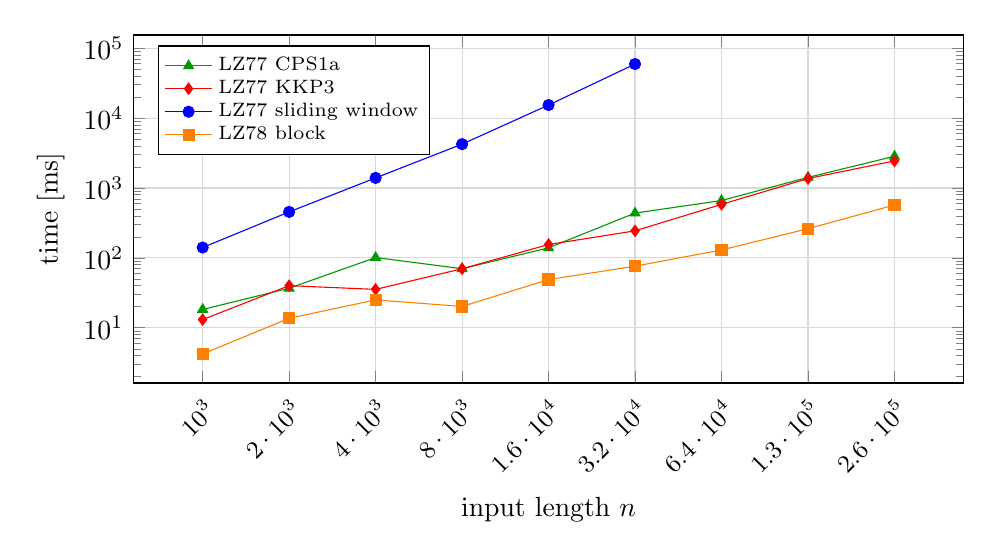
\begin{tikzpicture}
\begin{axis}[
  width = \linewidth, height = 6cm,
  xlabel = {input length $n$}, ylabel = {time [ms]},
  xmode = log, ymode = log,
  legend pos = north west, legend cell align = left,
  legend style = {font = \scriptsize, row sep = -2pt, inner sep = 2pt},
  xmajorgrids = true, ymajorgrids = true,
  xminorgrids = false, yminorgrids = false,
  minor tick num = 0,
  grid style = {draw = gray!30},
  xtick = {1000, 2000, 4000, 8000, 16000, 32000, 64000, 128000, 256000},
  xticklabels = {$10^{3}$, $2 \cdot 10^{3}$, $4 \cdot 10^{3}$, $8 \cdot 10^{3}$, $1.6 \cdot 10^{4}$, $3.2 \cdot 10^{4}$, $6.4 \cdot 10^{4}$, $1.3 \cdot 10^{5}$, $2.6 \cdot 10^{5}$},
  x tick label style = {rotate = 45, anchor = north east, font = \small},
]
\addplot[color = green!60!black, mark = triangle*] coordinates {(1000, 18.28) (2000, 36.78) (4000, 101.1) (8000, 69.96) (16000, 139.19) (32000, 437.01) (64000, 660.93) (128000, 1418.77) (256000, 2840.15)};
\addlegendentry{LZ77 CPS1a}
\addplot[color = red, mark = diamond*] coordinates {(1000, 13.09) (2000, 40.03) (4000, 35.41) (8000, 69.86) (16000, 155.27) (32000, 243.6) (64000, 582.68) (128000, 1365.72) (256000, 2436.28)};
\addlegendentry{LZ77 KKP3}
\addplot[color = blue, mark = *] coordinates {(1000, 140.51) (2000, 454.42) (4000, 1393.42) (8000, 4235.39) (16000, 15349.14) (32000, 59263.25)};
\addlegendentry{LZ77 sliding window}
\addplot[color = orange, mark = square*] coordinates {(1000, 4.22) (2000, 13.67) (4000, 25.07) (8000, 20.17) (16000, 48.93) (32000, 76.0) (64000, 129.77) (128000, 261.37) (256000, 570.51)};
\addlegendentry{LZ78 block}
\end{axis}
\end{tikzpicture}
\captionof{figure}{natural, encoding time.}
\label{fig:natural-encoding}
\end{center}

\begin{center}
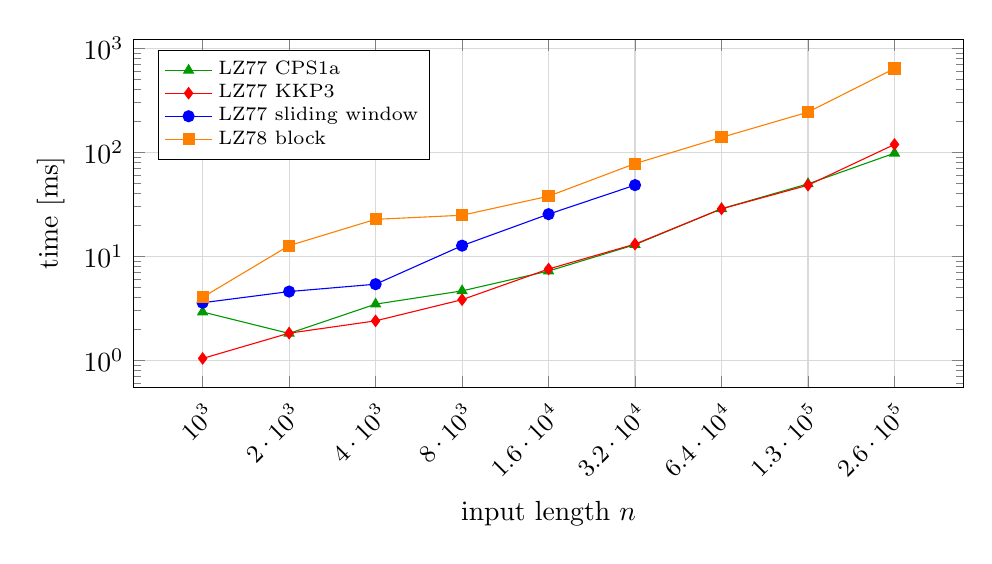
\begin{tikzpicture}
\begin{axis}[
  width = \linewidth, height = 6cm,
  xlabel = {input length $n$}, ylabel = {time [ms]},
  xmode = log, ymode = log,
  legend pos = north west, legend cell align = left,
  legend style = {font = \scriptsize, row sep = -2pt, inner sep = 2pt},
  xmajorgrids = true, ymajorgrids = true,
  xminorgrids = false, yminorgrids = false,
  minor tick num = 0,
  grid style = {draw = gray!30},
  xtick = {1000, 2000, 4000, 8000, 16000, 32000, 64000, 128000, 256000},
  xticklabels = {$10^{3}$, $2 \cdot 10^{3}$, $4 \cdot 10^{3}$, $8 \cdot 10^{3}$, $1.6 \cdot 10^{4}$, $3.2 \cdot 10^{4}$, $6.4 \cdot 10^{4}$, $1.3 \cdot 10^{5}$, $2.6 \cdot 10^{5}$},
  x tick label style = {rotate = 45, anchor = north east, font = \small},
]
\addplot[color = green!60!black, mark = triangle*] coordinates {(1000, 2.91) (2000, 1.81) (4000, 3.46) (8000, 4.64) (16000, 7.2) (32000, 12.91) (64000, 28.6) (128000, 49.59) (256000, 97.79)};
\addlegendentry{LZ77 CPS1a}
\addplot[color = red, mark = diamond*] coordinates {(1000, 1.04) (2000, 1.82) (4000, 2.39) (8000, 3.82) (16000, 7.53) (32000, 13.07) (64000, 28.51) (128000, 48.16) (256000, 118.66)};
\addlegendentry{LZ77 KKP3}
\addplot[color = blue, mark = *] coordinates {(1000, 3.57) (2000, 4.57) (4000, 5.38) (8000, 12.63) (16000, 25.35) (32000, 48.24)};
\addlegendentry{LZ77 sliding window}
\addplot[color = orange, mark = square*] coordinates {(1000, 4.03) (2000, 12.63) (4000, 22.62) (8000, 24.75) (16000, 37.74) (32000, 77.66) (64000, 138.71) (128000, 242.65) (256000, 636.97)};
\addlegendentry{LZ78 block}
\end{axis}
\end{tikzpicture}
\captionof{figure}{natural, decoding time.}
\label{fig:natural-decoding}
\end{center}

\begin{center}
\begin{tabular}{lrrrrrr}
\hline
algorithm & $n$ & $\alpha$ & $z$ & $\rho$ & encode [ms] & decode [ms] \\
\hline
LZ77 sliding window & 32000 & 34 & 6133 & 1.3416 & 55752.28 & 47.67 \\
LZ78 block & 32000 & 34 & 8078 & 0.8481 & 64.83 & 65.97 \\
LZ77 CPS1a & 32000 & 34 & 6133 & 0.9583 & 314.13 & 12.97 \\
LZ77 KKP3 & 32000 & 34 & 6133 & 0.9583 & 281.1 & 25.07 \\
\hline
\end{tabular}
\captionof{table}{natural: Pan Tadeusz, letters and spaces only.}
\label{tab:natural}
\end{center}